\section{Auswertung}
\label{sec:Auswertung}
\subsection{Messgrößen und Fehler}
Die Reserviore werden jeweils mit
\begin{equation}
  V_{\text{Reservior}} = 4 \text{L}
  \label{eqn:v}
\end{equation}
Wasser befüllt. Desweiteren werden die Temperatur $T_\text{1}$ und $T_\text{2}$, der Druck $p_{\text{b}}$ und $p_{\text{a}}$ sowie die Leistung des Kompressors jede Minute von den Messinstrumenten abgelesen. Die Messdaten werden in Tabelle \ref{tab:Daten} aufgelistet. Die Wärmekapazität der Reservoire beträgt
\begin{equation}
  C_{\text{Reservoire}} = 750 \frac{\text{J}}{\text{K}}
  \label{eqn:c_re}
\end{equation}

\begin{table}
  \centering
  \begin{tabular}{c c c c c c}
    \toprule
    $t$ / min & $T_\text{1}$ / K & $p_\text{b}$ / kPa & $T_\text{2}$ / K & $P_\text{a}$ / kPa & Leistung / kW \\
    \midrule
    0 	& 294.1 & 466	& 294.3	& 496	& 0	    \\
    1 	& 294.7 & 608	& 294.3	& 425	& 1.18	\\
    2 	& 295.9 & 618	& 293.2	& 446	& 1.2	  \\
    3 	& 296.9 & 638	& 292.5	& 466	& 1.25	\\
    4	  & 298.2	& 628	& 291.3	& 466	& 1.25	\\
    5	  & 299.4 & 709	& 290.2	& 466	& 1.25	\\
    6	  & 300.7 & 730	& 289.3	& 466	& 1.25	\\
    7	  & 302.0 & 760	& 288.5	& 455	& 1.25	\\
    8	  & 303.2	& 790	& 287.7	& 445	& 1.25	\\
    9	  & 304.4 & 812	& 287.0	& 425	& 1.24	\\
    10	& 305.5 & 820	& 286.3	& 425	& 1.24	\\
    11 	& 306.6 & 840	& 285.6	& 415	& 1.23	\\
    12	& 307.6	& 861	& 284.9	& 405	& 1.23	\\
    13	& 308.7 & 891	& 284.1	& 405	& 1.23	\\
    14 	& 309.7 & 911	& 283.5	& 395	& 1.23	\\
    15 	& 310.7 & 922	& 282.8	& 395	& 1.24	\\
    16 	& 311.6	& 963	& 282.2	& 385	& 1.25	\\
    17	& 312.5	& 993	& 281.5	& 385	& 1.25	\\
    18	& 313.5	& 1003	& 281.0	& 375	& 1.25	\\
    19	& 314.3	& 1023	& 280.5	& 365	& 1.25	\\
    20	& 315.2	& 1044	& 280.0	& 365	& 1.25	\\
    21	& 316.0	& 1064	& 279.5	& 365	& 1.25	\\
    22	& 316.8	& 1094	& 279.0	& 365	& 1.25	\\
    23	& 317.5	& 1104	& 278.6	& 355	& 1.25	\\
    24	& 318.3	& 1115	& 278.3	& 355	& 1.25	\\
    25	& 319.0	& 1135	& 277.9	& 355	& 1.25	\\
    26	& 319.8	& 1155	& 277.5	& 345	& 1.25	\\
    27	& 320.5	& 1175	& 277.2	& 345	& 1.25	\\
    28	& 321.2	& 1196	& 276.9	& 345	& 1.25	\\
    29	& 321.8	& 1216	& 276.6	& 345	& 1.25	\\
    30	& 322.5	& 1226	& 276.3	& 345	& 1.25	\\
    31	& 323.3	& 1236	& 276.1	& 354	& 1.25	\\
  \end{tabular}
  \caption{Dem Versuchsaufbau entommene Messgrößen}
  \label{tab:Daten}
\end{table}

Zu beachten ist das alle Messgrößen einen Messunsicherheit besitzen, einerseits eine Ablesefehler bei analogen Messinstrumenten als auch einen Technischen.
\begin{eqnarray*}
  \Delta p =& &\pm 10 \text{kp}				\\
  \Delta C =& &\pm 10 \frac{\text{J}}{\text{K}}		\\
  \Delta V =& &\pm 1.6 \text{mL}				\\
  \Delta \rho =& &\pm 13 \frac{\text{kg}}{\text{m$^2$}}	\\
\end{eqnarray*}
Die Messunsicherheit der Dichte für Wasser kommt daraus zu stande, dass Wasser bei verschiedenen Temperaturen seine Dichte ändert.
\begin{figure}
  \centering
  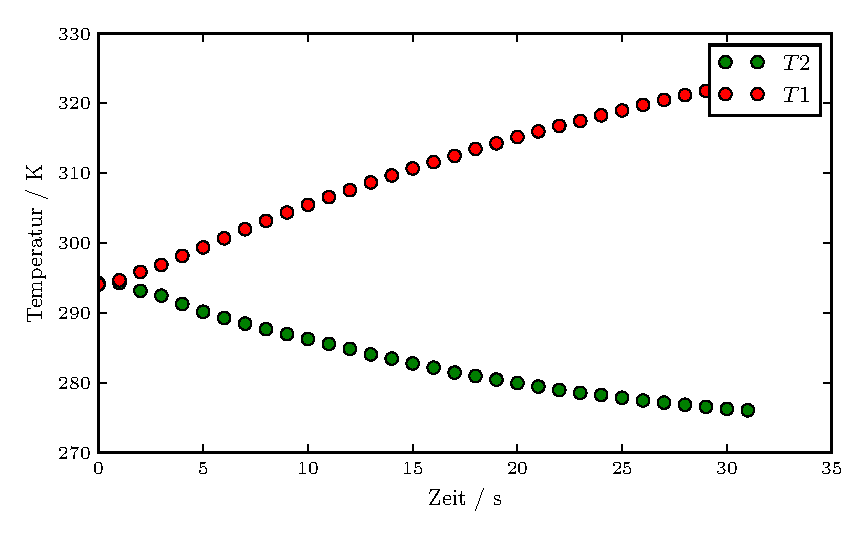
\includegraphics[width=\textwidth]{TVerlauf.pdf}
  \caption{Temperaturverläufe $T_\text{1}$ und $T_\text{2}$}
  \label{fig:T1&T2}
\end{figure}
\subsection{Näherungsfunktion}
Mit einer nicht-linearen Ausgleichsgraden soll der Temperaturverlauf mit Hilfe der Gleichung ?? approximiert werden. Eine Approximation soll mittels eines Polynoms 2-Grades erfolgen.
\begin{equation}
  T(t) = At^2 + Bt +C
  \label{eqn:ausgleichsgrade}
\end{equation}
Die Ermittelung der Ausgleichsgraden erfolgt mit hilfe von Python 3.4.3.
\begin{figure}
  \centering
  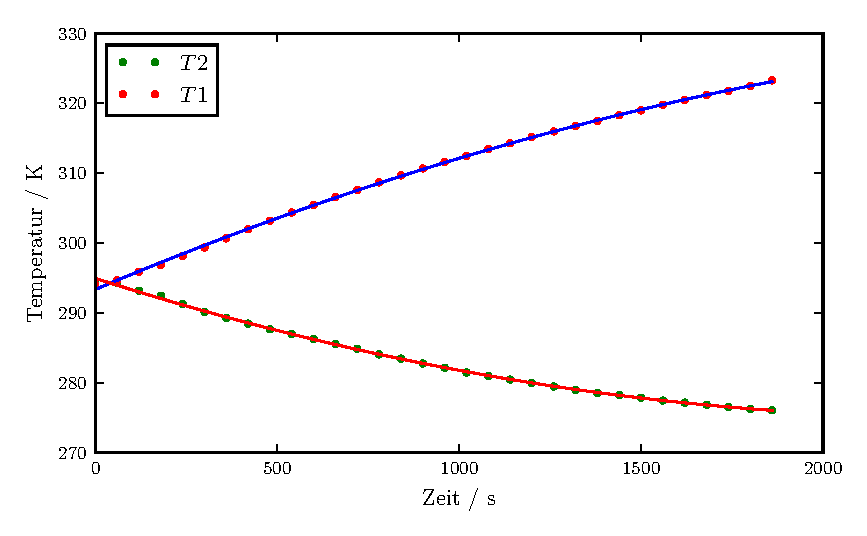
\includegraphics[width=\textwidth]{Ausgleichsgrade.pdf}
  \caption{nicht-lineare Ausgleichsgrade}
  \label{fig:ausg}
\end{figure}
Mittels einer fit Funktion werden die Koeffizienten bestimmt. Für die Temperatur $T_\text{1}$ ergeben sich die Koeffizienten
\begin{eqnarray}
  A =& -3.23 \cdot 10^{-6} \, \frac{\text{K}}{\text{s}^2}	\\
  B =& 2.20 \cdot 10^{-2} \, \frac{\text{K}}{\text{s}} 	\\
  C =& 2.93 \cdot 10^{2} \, \text{K} \\
  \label{eqn:koefT1}
\end{eqnarray}
und für $T_\text{2}$
\begin{eqnarray}
  A =& 3.49 \cdot 10^{-6} \, \frac{\text{K}}{\text{s}^2} 	\\
  B =& -1.67 \cdot 10^{-2} \, \frac{\text{K}}{\text{s}} 	\\
  C =& 2.94 \cdot 10^2 \, \text{K}
  \label{eqn:koefT2}
\end{eqnarray}
Dabei wird vernachlässigt das die Koeffizienten Fehlerbehaftet sind, weil dies nicht mittels fit Funktion ermittelt werden kann.
\subsection{Differentialquotient}
Der Differentialquotient berechnet sich aus einmaligen Ableiten der Gleichung \ref{eqn:ausgleichsgrade} nach der Zeit.
\begin{equation}
  \frac{dT_\text{i}}{dt} = 2At + B
  \label{eqn:diffq}
\end{equation}
Aus der Funktion wird der Differentialqutient für $T_\text{1}$ und $T_\text{2}$ für vier verschieden Zeiten berechnet. Die Ergebnisse sind in Tabelle \ref{tab:diffQ} aufgeführt.
\begin{table}
  \centering
  \begin{tabular}{c c c c c}
  	\toprule
	t / s & $T_\text{1}$ / K & $\frac{dT1}{dt}$ / $10^{-2}$ s/K & $T_\text{2}$ / K & $\frac{dT2}{dt}$ / $10^{-2}$ s/K \\
	\midrule
	60	  & 294.7   & 2.16 & 294.0 & -1.62 \\
	400	  & 301.7   & 1.94 & 288.9 & -1.35 \\
	1000	& 312.2   & 1.55 & 281.8 & -0.97 \\
	1500	& 319.1   & 1.23 & 277.9 & -0.62 \\
	\bottomrule
  \end{tabular}
  \caption{Differentialqoutient für $T_\text{1}$ und $T_\text{2}$}
  \label{tab:diffQ}
\end{table}

\subsection{Güteziffer}
Mit Hilfe des Differentialqoutienten und der Wärmekapazität der mit Wasser befüllten Reservoire
\begin{equation}
  c_\text{w} m_\text{w} = 6230.64 \cdot (\num{4000 +- 1.6}) \, \frac{\text{J}}{\text{K}} = (\num{24.9 +- 0.0}) \cdot 10^6 \, \frac{\text{J}}{\text{K}}
  \label{eqn:WC}
\end{equation}
soll die Güteziffer des Versuches bestimmt werden. Die Theoretische Güteziffer lässt sich mit hilfe der Gleichung \ref{eqn:nureal} berechnen und ist in Tabelle \ref{tab:gueteziffer} aufgeführt. Die praktisch bestimmte Güteziffer errechnet sich nach Gleichung \ref{eqn:nureal} aus der Wärmekapazität der Reservoire und der Wärmekapazität der Leitungen
\begin{equation}
  c_\text{k} m_\text{k} = (\num{750 +- 10}) \, \frac{\text{J}}{\text{K}} \ ,
  \label{eqn:Res}
\end{equation}
sowie denn in Tabelle 1 bestimmten Differentialquotienten, so wie der nach Formel \ref{eqn:ave} und \ref{eqn:var} gemittelte Leistung.
\begin{table}
  \centering
  \begin{tabular}{c c c}
    \toprule
    $t$ / s & $\nu_\text{theo}$ & $\nu_\text{exp}$ \\
    \midrule
    60	 & 421.0 & \num{3.2 +- 0.6} 	\\
    400  & 23.6	 & \num{2.8 +- 0.5} 	\\
    1000 & 10.3	 & \num{2.3 +- 0.4}	\\
    1500 & 7.6	 & \num{1.8 +- 0.3} 	\\
    \bottomrule
  \end{tabular}
  \caption{theoretisch und praktisch bestimmte Güteziffer}
  \label{tab:gueteziffer}
\end{table}
Gründe für die Abweichung zwischen der theoretischen Güteziffer und der experimentell ermittelten Güteziffer werden in der Diskussion aufgeführt.
\subsection{Dampfdruckkurve}
Die Verdampfungswärme $L$ wird mit einer Verdampfungskurve ermittelt. Dafür wird im Diagramm \ref{fig:dampfdruck}
\begin{figure}
  \centering
  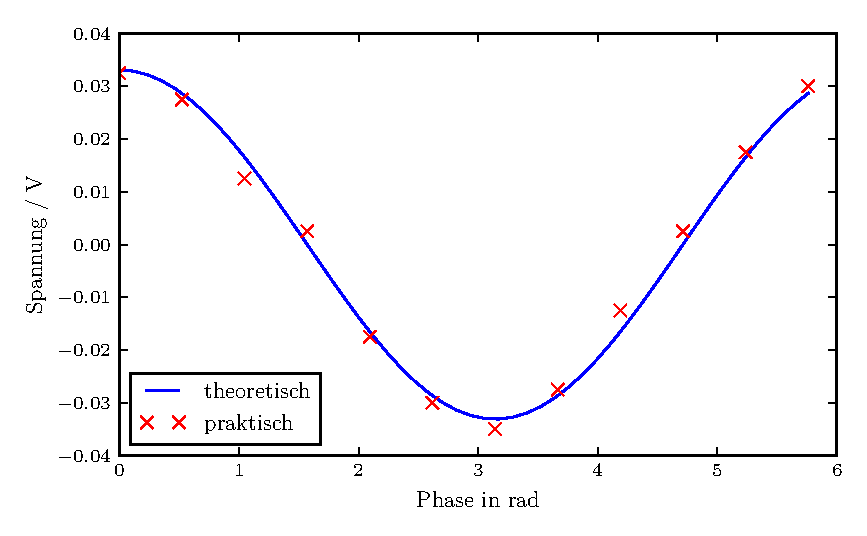
\includegraphics[width=\textwidth]{Dampfdruck.pdf}
  \caption{Dampfdruckkurve}
  \label{fig:dampfdruck}
\end{figure}
$1/T$ gegen $log(p/p_0)$ aufgetragen und in die Steigung der Graden in die Formel \ref{eqn:damüfgl} eingesetzt.
\begin{equation}
  L = log \left( \frac{p}{p_o} \right) \cdot T \cdot \frac{1}{R}
  \label{eqn:dampfgl}
\end{equation}
Die Steigung der Ausgleichsgraden wird mittels einer linearen Regression berechnet und beträgt
\begin{equation*}
  m = \num{-2430 +- 20} \ .
\end{equation*}
Daraus ergibt sich eine Verdampfungswärme von
\begin{equation}
  L = (\num{20200 +- 170}) \, \frac{\text{Js}}{\text{molK}} \ .
\end{equation}
\subsection{Massendurchsatz}
Die Verdampfungswärme wird nun in Formel ?? eingesetzt und damit der Massendurchsatz ermittelt. Die Massendurchsätze der verschiedenen Zeiten sind in Tabelle \ref{tab:dm/dt} aufgetragen.
\begin{table}
  \centering
  \begin{tabular}{c c c}
    \toprule
    $T$ / s & $\frac{dm}{dt}$ / (mol/s) & $\frac{dm}{dt}$ / (g/s) \\
    \midrule
    60   & \num{0.0140 +- 0.001} & \num{1.69 +- 0.1}\\
    400  & \num{0.0120 +- 0.001} & \num{1.45 +- 0.1}\\
    1000 & \num{0.0083 +- 0.001} & \num{1.00 +- 0.1}\\
    1500 & \num{0.0053 +- 0.001} & \num{0.64 +- 0.1}\\
    \bottomrule
  \end{tabular}
  \caption{Massendurchsatz $dm/dt$}
  \label{tab:dm/dt}
\end{table}
Für die weiteren Rechnungen wird der Massendurchsatz durch Multiplikation mit der Molaren Masse in die SI-Einheit umgerechent.
\subsection{mechanische Kompressorleistung}
Aus der idealen Gasgleichung lässt sich die Dichte in den Rohren berechnen. Dafür muss jedoch die Dichte von Dichlorfluormethan bei 1 Bar Druck und 273 Kelvin bekannt sein.
\begin{equation}
  \rho_\text{0} =  5.51 \frac{\text{g}}{\text{l}} \ .
  \label{rho}
\end{equation}
Zusätzlich wird gefordert, dass
\begin{equation}
  nR = konstant
\end{equation}
ist und das die Dichte homogen verteilt ist. Daraus lässt sich die Ideale Gasgleichung umstellen und man erhält
\begin{eqnarray*}
  \frac{pV}{T} =nR =& konst \\
  \frac{p_0 V_0}{T_0} = \frac{p_2 V_2}{T_\text{2}}  \Leftrightarrow&  \frac{p_0 m}{\rho_0 T_0} = \frac{p_2 m}{T_\text{2} \rho_2} \\
  \frac{p_0}{\rho_0 T_0} = \frac{p_2}{T_\text{2} \rho} \Leftrightarrow& \rho = \frac{\rho_o T_o P_2}{T_\text{2} P_0}
  \label{eqn:rho}
\end{eqnarray*}
einen Ausdruck für die Dichte in Abhängingkeit der Temperaturen und Drücke.
